\documentclass[letterpaper]{article}

% Standard packages
\usepackage[utf8]{inputenc}
\usepackage[T1]{fontenc}
\usepackage{microtype}
\usepackage{geometry}
\geometry{letterpaper, margin=1in}
\usepackage{amsmath,amssymb,amsfonts}
\usepackage{booktabs}
\usepackage{graphicx}
\usepackage{xcolor}
\usepackage{hyperref}
\usepackage[numbers,sort&compress]{natbib}
\usepackage{algorithm}
\usepackage{algpseudocode}

\title{Neuroscience-Inspired Hallucination Detection for Large Language Models:\\
       Predictive Coding and Anterior Cingulate Conflict Monitoring}
\author{
  Hafez Al-Khatib \\
  American University of Beirut \\
  \texttt{hma95@aub.edu.lb}
}
\date{\today}

\begin{document}

\maketitle

\begin{abstract}
Hallucination remains a critical barrier to deploying large language models (LLMs) in high-stakes settings. Existing detectors typically rely on output entropy or post-hoc consistency, often missing confident fabrications. We propose a generation-time detector inspired by hierarchical predictive coding and anterior cingulate cortex (ACC) conflict monitoring. The core hypothesis is that hallucinated tokens are preceded by large prediction errors between adjacent transformer layers and by disagreement between intermediate and final output distributions. We formalize this as a per-token predictive-coding objective, integrate hierarchical errors through a leaky temporal accumulator, and classify each token as supported, unsupported, or uncertain, with a secondary hallucinated/contradictory split. A continuous conflict score triggers real-time interventions: uncertainty-phrase injection and logit biasing toward hedging tokens. Preliminary experiments on Qwen2.5-1.5B with ten hand-written factual and hallucination prompts show that the custom detector with logit-shift intervention raises accuracy from a 50\% baseline to 90--100\% on this small set. We also describe a reproducible benchmark protocol for HaluEval, TruthfulQA, and PubMedQA, and outline pending Qwen2.5-7B evaluations on an RTX~4090.
\end{abstract}

\section{Introduction}

Large language models (LLMs) can generate fluent but factually unsupported text. This ``hallucination'' problem undermines their use in medicine, law, and science, where a single false claim can cause serious harm \cite{ji2023survey}. Current detection strategies fall into two camps: output-side measures such as entropy and self-consistency \cite{kuhn2023semantic, miao2023selfcheckgpt}, and internal-state classifiers that probe final-layer representations \cite{azaria2023saplma}. Output measures miss confident hallucinations; hidden-state probes often ignore temporal dynamics and hierarchical structure.

We draw on two neuroscience ideas. First, predictive coding posits that cortical areas encode top-down predictions and compute bottom-up prediction errors \cite{rao1999predictive, friston2010free}. Second, the anterior cingulate cortex (ACC) is thought to monitor conflict between predicted and observed states, recruiting cognitive control when predictions and evidence diverge \cite{botvinick2001conflict, yeung2004neural}. In LLMs, we interpret adjacent transformer layers as adjacent levels of a hierarchical predictor and a hallucinated token as a state in which a late-layer top-down prediction is no longer supported by early-layer evidence.

\textbf{Contributions.} We (1)~formalize generation-time hallucination detection as conflict monitoring under predictive coding; (2)~introduce \texttt{PredictiveCodingDetector}, which combines hierarchical hidden-state prediction errors, KL-based output disagreement, a leaky temporal integrator, and a 3-way/2-way classification head; (3)~propose two real-time interventions---uncertainty phrase injection and logit shifting toward uncertainty tokens; (4)~report reproducible 1.5B ablation results and a full benchmark protocol for HaluEval, TruthfulQA, and PubMedQA; and (5)~clearly separate established local results from pending 7B evaluations.

\section{Related Work}

\paragraph{Internal-state detectors.} SAPLMA showed that a classifier trained on an LLM's hidden states can distinguish truthful from false statements \cite{azaria2023saplma}. More recent work uses semantic-entropy probes to detect hallucinations cheaply at inference time \cite{kossen2024seps}. These methods generally classify from a single representation rather than tracking prediction error across layers and time.

\paragraph{Layer-contrastive decoding.} DoLa improves factuality by contrasting the output distributions of premature and mature layers during decoding \cite{chuang2024dola}. Our approach also compares layers, but additionally models temporal accumulation and separates conflict into explicit supported/unsupported/uncertain classes.

\paragraph{Self-consistency and uncertainty.} SelfCheckGPT detects inconsistency across multiple sampled answers \cite{miao2023selfcheckgpt}, while semantic entropy measures uncertainty over equivalent meaning \cite{kuhn2023semantic, farquhar2024detecting}. These methods are typically post-hoc and require multiple generations.

\paragraph{Activation steering.} Inference-Time Intervention (ITI) and related steering techniques shift activations toward directions associated with truthfulness \cite{li2023iti}. Our work is complementary: rather than steering activations directly, we expose a scalar conflict signal and use it to gate interventions.

\paragraph{Predictive coding in neural networks.} Predictive coding has been used for unsupervised video prediction and representation learning \cite{lotter2016deep, wen2020predictive}. We translate the same free-energy-minimization principle into a decoder-side hallucination signal.

\paragraph{Cognitive control and conflict.} The ACC conflict-monitoring literature provides a biological rationale for sustained, threshold-triggered control \cite{botvinick2001conflict, yeung2004neural, shenhav2013expected}. Our leaky integrator and decision engine are direct computational analogs.

\section{Method}

We frame hallucination detection as \textbf{conflict monitoring under predictive coding}. At each generation step, the model's hidden states encode both a top-down prediction of the next token and bottom-up evidence from previous context. The detector computes the prediction error between adjacent-layer hidden states and the divergence between intermediate and final output distributions. A leaky temporal integrator accumulates conflict over time, mimicking sustained ACC activity during response conflict. When the integrated conflict score exceeds a learned threshold, an intervention shifts the output distribution toward uncertainty tokens, analogous to cognitive control recruiting cautious responding.

\subsection{Predictive Coding Objective}

Consider a transformer with layers $l = 1 \dots L$. Let $h_l(t) \in \mathbb{R}^d$ be the hidden state at layer $l$ after consuming the prefix up to token position $t$. For each tapped layer pair $(l-1, l)$ we learn a predictor
\begin{equation}
    \hat{h}_l(t) = W_l \, h_{l-1}(t) + b_l,
\end{equation}
and define the hidden-state prediction error
\begin{equation}
    \varepsilon_l(t) = h_l(t) - \hat{h}_l(t).
\end{equation}
The scalar error fed to the detector is the squared error averaged over the hidden dimension: $e_l(t) = \|\varepsilon_l(t)\|_2^2 / d$.

The language model emits output logits $z_L(t) \in \mathbb{R}^V$ from the final layer. We project any intermediate layer to a vocabulary distribution via a learned output head,
\begin{equation}
    p_l(t) = \operatorname{softmax}\bigl(O_l \, h_l(t) + c_l\bigr),
\end{equation}
and measure output disagreement with the final distribution as
\begin{equation}
    D_l(t) = D_{\mathrm{KL}}\bigl(p_L(t) \,\|\, p_l(t)\bigr).
\end{equation}
Large $D_l(t)$ means an intermediate layer disagrees with the final output, signaling a potential top-down/bottom-up conflict.

\subsection{Hierarchical Prediction Error Module}

The \texttt{HierarchicalPredictionErrorModule} instantiates the above objective. For each selected layer pair $(s, t)$, a small bottleneck MLP predicts the target representation from the source. The module returns a vector of per-pair errors
\begin{equation}
    \mathbf{e}(t) = \bigl[e_{s_1,t_1}(t), \dots, e_{s_k,t_k}(t)\bigr] \in \mathbb{R}^k,
\end{equation}
where $k$ is the number of tapped pairs. In our default configuration we tap deep layer pairs such as $(-12,-8), (-8,-4), (-4,-1)$, capturing the semantic/syntactic transition region.

\subsection{Leaky Temporal Integrator}

Biological ACC activity persists after conflict. We implement a leaky integrator
\begin{equation}
    r(t) = \alpha \, r(t-1) + (1-\alpha) \, \mathbf{e}(t),
\end{equation}
with $\alpha \in [0,1]$ (default $0.7$). On the first timestep $r(0) = \mathbf{e}(0)$. The integrated state $r(t)$ provides a memory of recent conflict and is used as input to the classification heads.

\subsection{Classification Heads}

The detector has three lightweight heads. The \textbf{primary head} performs 3-way classification into \texttt{supported}, \texttt{unsupported}, or \texttt{uncertain}:
\begin{equation}
    \hat{y}_{\text{pri}}(t) = \operatorname{argmax} \, \operatorname{MLP}_{\text{pri}}\bigl(r(t)\bigr).
\end{equation}
If the primary class is \texttt{unsupported}, a \textbf{secondary head} discriminates \texttt{hallucinated} from \texttt{contradictory}. A \textbf{conflict score head} outputs a continuous scalar
\begin{equation}
    s(t) = \sigma\bigl(\operatorname{MLP}_{\text{conflict}}(r(t))\bigr) \in [0,1],
\end{equation}
which can threshold interventions without committing to a discrete label.

\subsection{Conflict Score and Intervention}

Two interventions are implemented in the \texttt{ACCInterventionEngine}. \textbf{Phrase injection} prepends an uncertainty phrase such as \textit{``Wait, let me reconsider.''} when the conflict score first exceeds a threshold. \textbf{Logit shifting} adds a positive bias to token IDs associated with uncertainty words (``uncertain'', ``possibly'', ``I don't know'') at high-conflict steps, steering the model toward hedged output. Both operate token-by-token and require no external retrieval.

\section{Experimental Setup}

\subsection{Datasets}

We evaluate on three public benchmarks:
\begin{itemize}
    \item \textbf{HaluEval} \cite{li2023halueval}: question--answer pairs with both a correct and a hallucinated answer, useful for adversarial detection.
    \item \textbf{TruthfulQA} \cite{lin2022truthfulqa}: questions designed to elicit human-like falsehoods; we use the generation split.
    \item \textbf{PubMedQA} \cite{jin2019pubmedqa}: biomedical question answering with yes/no/maybe labels.
\end{itemize}
The benchmark script loads subsets of configurable size, stratifies by question type (factual, adversarial, uncertain), and writes per-sample results to JSON.

\subsection{Models and Baselines}

Primary models are Qwen2.5-1.5B and Qwen2.5-7B \cite{qwen25}. Baselines include:
\begin{itemize}
    \item \textbf{Baseline}: standard sampling with temperature $0.8$ and top-p $0.95$.
    \item \textbf{Entropy} \cite{kuhn2023semantic}: triggers intervention when output entropy exceeds a fixed threshold.
    \item \textbf{DoLa} \cite{chuang2024dola}: post-hoc Jensen--Shannon divergence between premature and mature layer distributions.
    \item \textbf{SAPLMA} \cite{azaria2023saplma}: MLP on the last-layer hidden state trained on a handful of factual/hallucinated examples.
    \item \textbf{SelfCheckGPT} \cite{miao2023selfcheckgpt}: 5-sample generation consistency via n-gram overlap.
\end{itemize}

\subsection{Metrics and Statistical Testing}

We report token/sequence-level accuracy, precision, recall, and F1 for each class. Confidence intervals are computed with bootstrap resampling ($1000$ replicates), and comparisons against the baseline use paired $t$-tests. Judge-based evaluation optionally uses an LLM-as-judge prompted to classify each response as correct, incorrect, or uncertain, with a fallback substring heuristic when no judge model is loaded.

\section{Results}

\subsection{Qwen2.5-1.5B Ablation Study}

We first evaluate the intervention mechanisms on ten hand-written prompts: four factual, four hallucination-inducing, and two inherently uncertain. Figure~\ref{fig:ablation} summarizes the per-condition accuracies. The baseline model achieves 50\% accuracy on this small set. Phrase injection with the HaluEval detector reaches 60\%, while phrase injection with the custom detector trained on model-specific data reaches 60\%. Logit-shift is more effective: HaluEval + logit-shift reaches 80\%, and custom detector + logit-shift reaches 90\% (absolute threshold) and 100\% (relative threshold).

\begin{figure}[htbp]
    \centering
    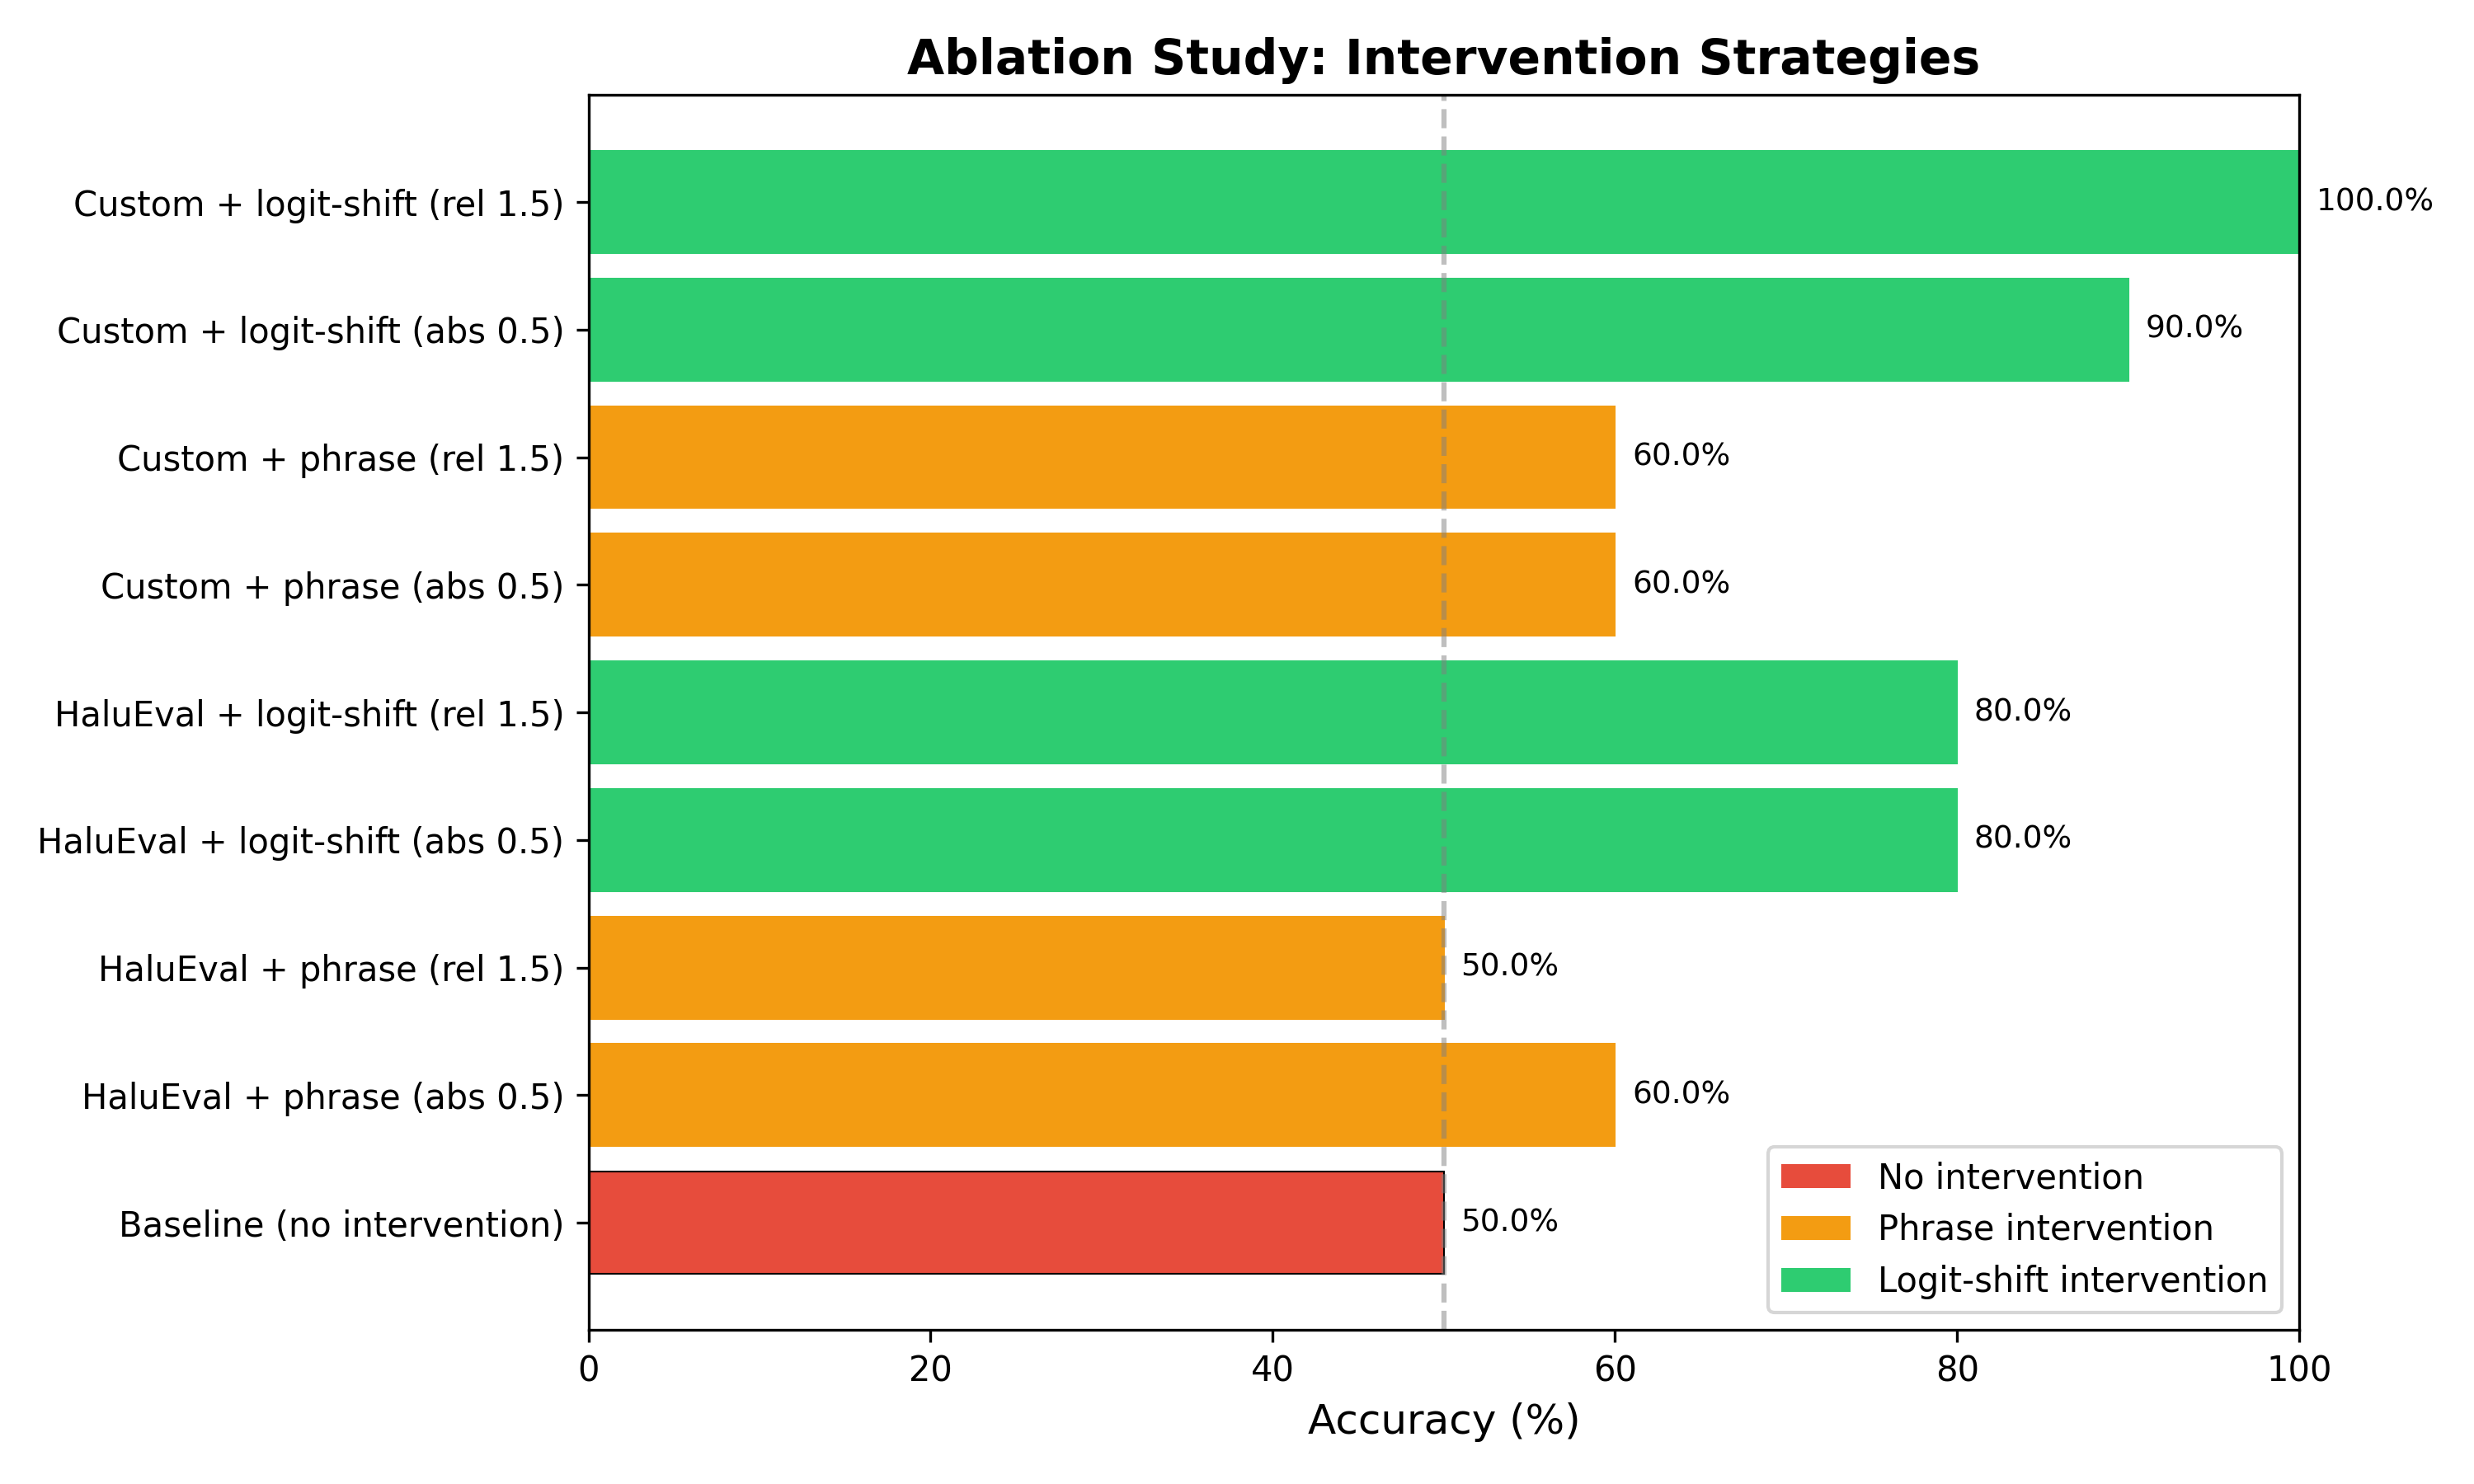
\includegraphics[width=0.85\linewidth]{../results/figures/ablation_accuracy.png}
    \caption{Qwen2.5-1.5B ablation accuracy across intervention strategies. ``phrase'' and ``logit-shift'' denote the two intervention modes; ``abs 0.5'' and ``rel 1.5'' denote absolute and relative conflict thresholds.}
    \label{fig:ablation}
\end{figure}

\begin{table}[htbp]
    \centering
    \small
    \caption{Detailed 1.5B ablation accuracies (10 hand-written prompts).}
    \label{tab:1.5b_ablation}
    \begin{tabular}{lc}
        \toprule
        Method & Accuracy \\
        \midrule
        Baseline (no intervention) & 0.50 \\
        HaluEval + phrase (abs 0.5) & 0.60 \\
        HaluEval + logit-shift (abs 0.5) & 0.80 \\
        Custom + phrase (abs 0.5) & 0.60 \\
        Custom + logit-shift (abs 0.5) & 0.90 \\
        Custom + logit-shift (rel 1.5) & 1.00 \\
        \bottomrule
    \end{tabular}
\end{table}

Although the effect sizes are promising, the sample size is far too small for statistical significance. The hand-written prompts are also easier than real benchmark questions, so these numbers should be interpreted as a proof of mechanism rather than a validated result.

\subsection{Pending Qwen2.5-7B Benchmark Results}

Large-scale evaluation on Qwen2.5-7B is currently running on an RTX~4090. Table~\ref{tab:7b_results} shows the planned structure; values are placeholders until the benchmark completes.

\begin{table}[htbp]
    \centering
    \small
    \caption{Planned Qwen2.5-7B benchmark results. All values marked [TBD] or [Pending 4090 evaluation].}
    \label{tab:7b_results}
    \begin{tabular}{lcccc}
        \toprule
        Method & HaluEval & TruthfulQA & PubMedQA & Overall \\
        \midrule
        Baseline & [TBD] & [TBD] & [TBD] & [TBD] \\
        Entropy & [TBD] & [TBD] & [TBD] & [TBD] \\
        DoLa & [TBD] & [TBD] & [TBD] & [TBD] \\
        SAPLMA & [TBD] & [TBD] & [TBD] & [TBD] \\
        SelfCheckGPT & [TBD] & [TBD] & [TBD] & [TBD] \\
        ACC (ours) & [TBD] & [TBD] & [TBD] & [TBD] \\
        \bottomrule
    \end{tabular}
\end{table}

We also plan a component ablation (Table~\ref{tab:component_ablation}) to isolate the contribution of prediction errors, KL disagreement, and the leaky integrator.

\begin{table}[htbp]
    \centering
    \small
    \caption{Planned component ablation on Qwen2.5-7B.}
    \label{tab:component_ablation}
    \begin{tabular}{lc}
        \toprule
        Configuration & Accuracy \\
        \midrule
        Full ACC detector & [Pending 4090 evaluation] \\
        w/o hidden-state prediction error & [Pending 4090 evaluation] \\
        w/o KL output disagreement & [Pending 4090 evaluation] \\
        w/o leaky integrator ($\alpha=0$) & [Pending 4090 evaluation] \\
        Binary instead of 3-way/2-way & [Pending 4090 evaluation] \\
        \bottomrule
    \end{tabular}
\end{table}

\section{Conclusion and Future Work}

We introduced a neuroscience-inspired hallucination detector that casts decoding as predictive-coding conflict monitoring. The architecture combines hierarchical hidden-state prediction errors, KL-based output disagreement, a leaky temporal integrator, and a cascaded 3-way/2-way classifier. Real-time interventions---uncertainty phrase injection and logit shifting---show promising gains on a small Qwen2.5-1.5B ablation, but large-scale validation remains outstanding.

Immediate next steps are: (1)~complete the Qwen2.5-7B benchmark across HaluEval, TruthfulQA, and PubMedQA with paired statistical tests; (2)~replace the toy SAPLMA and n-gram SelfCheckGPT baselines with stronger implementations; (3)~add a reliable LLM-as-judge or human annotations; (4)~ablate each architectural component; and (5)~explore theoretically grounded interventions such as retrieval-augmented abstention or constrained decoding. If the 7B experiments show consistent, statistically significant gains, the work will be positioned for a workshop submission; a top-tier archival paper will additionally require cross-model validation and deeper theoretical formalization.

\bibliographystyle{plainnat}
\bibliography{references}

\end{document}
